\documentclass[12pt]{article}
\usepackage[top=1in,bottom=1in,left=1in,right=1in]{geometry}
\usepackage{alltt}
\usepackage{array}	
\usepackage{graphicx}
\usepackage{tabularx}
\usepackage{verbatim}
\usepackage{setspace}
\usepackage{listings}
\usepackage{amssymb,amsmath, amsthm}
\usepackage{qtree}
\usepackage{hyperref}
\usepackage{oz}
\usepackage[cc]{titlepic}
\usepackage{fancyvrb}
\usepackage{epstopdf}
\usepackage{soul}
\graphicspath{ {./figures/} }

\title{Concordia University\\
Department of Computer Science and Software Engineering\\
\textbf{SOEN 331-S: Formal Methods\\for Software Engineering}\\
\ \\
\textbf{Template for Assignment 4:\\Temporal Logic}}
\author{\textbf{Witnick-Hans Joseph}\\
		\texttt{ID: 29348743}\\
		\textbf{Alexandra Zana}\\
		\texttt{ID: 40131077}\\
		\textbf{Alexandre Eid}\\
		\texttt{ID: 40155833}
\ \\}
\date{\today}

\begin{spacing}{1.5}
\begin{document}
\maketitle

\newpage

\section{Problem 1 (46 pts): Analyzing program behavior}

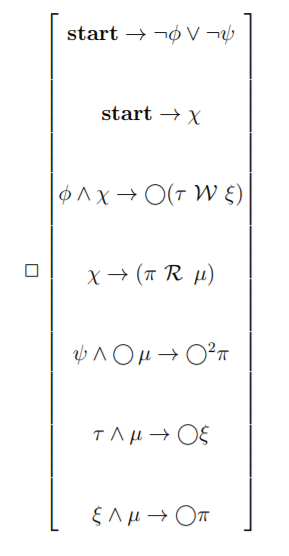
\includegraphics{p1-model.png}

\begin{enumerate}

	\item (36 pts) Visualize all models of behavior.

	\item (10 pts) Specify conditions (models of behavior), if any exist, under which the program\
	can terminate. If none exist, please indicate so.
		
\end{enumerate}

\begin{figure}[ht]
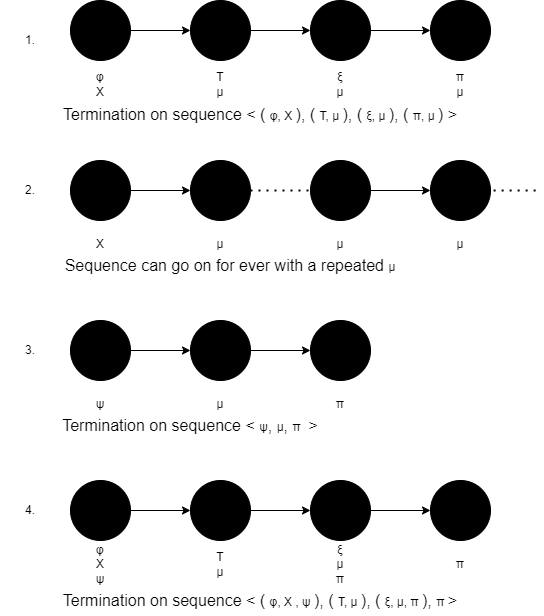
\includegraphics[scale=0.725]{p1.png}
\end{figure}
\newpage

\section{Problem 2 (54 pts) \\Interpreting and visualizing temporal expressionsogram behavior}

Interpret and visualize each of the following temporal expressions:

\begin{enumerate}

	\item $\Box \phi \rightarrow \bigcirc \psi $
	
		\noindent If $\phi$ is an invariant, then $\psi$ becomes true at i + 1.\\
		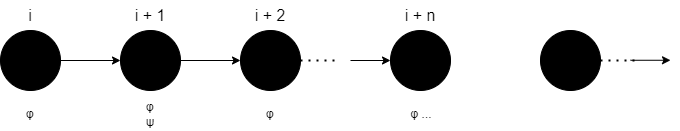
\includegraphics[scale=0.5]{p2.1.png}

	\item $\Box \phi \rightarrow \bigcirc \Diamond \Box \psi$
		
		\noindent If $\phi$ is an invariant, then $\psi$ starting from the next moment i+1 will eventually be true infinitely often.\\
		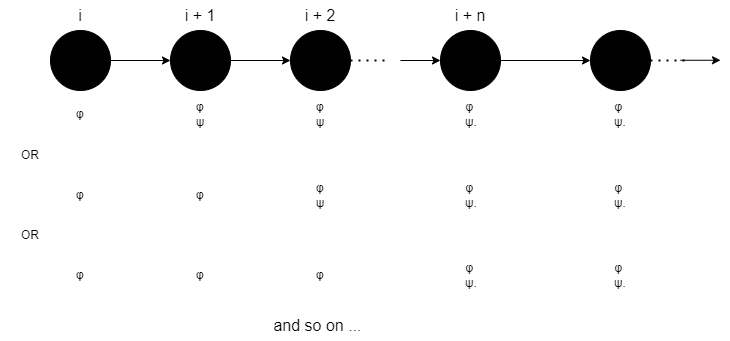
\includegraphics[scale=0.55]{p2.2.png}

	\item $(\phi \wedge \bigcirc \psi) \rightarrow \bigcirc \Box \chi $	

	
		\noindent If $phi$ is true at time = $i$ and $\psi$ is true at time = $i + 1$,
				$\tau$ becomes true and stays true at time i+1.\\
		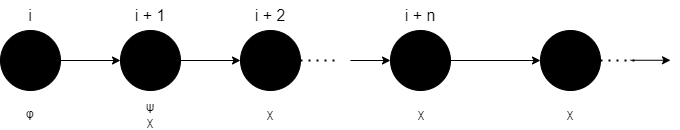
\includegraphics[scale=0.55]{p2.3.png}
	
	\item $( \psi \wedge \psi) \rightarrow \phi \mathcal{W} \tau \Longleftrightarrow
	 \psi \rightarrow \phi \mathcal{W} \tau$


		\noindent If $\psi$ is true at time = $i$ ,\
			then $\psi$ is also true at time $i$ and remains true up until(but not including) the moment $\tau$ first becomes true. $\tau$ may never become true.\\
		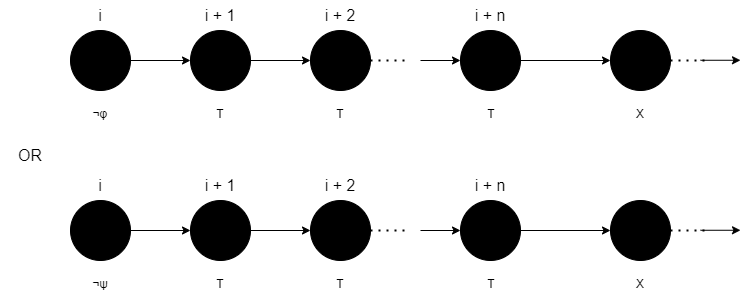
\includegraphics[scale=0.55]{p2.5.png}
	
	\item $( \lnot \phi \wedge \lnot \psi ) \rightarrow \bigcirc \tau \mathcal{U} \chi ?$ Explain your reasoning.

	
	\item Is the previous expression semantically equivalent to $( \phi \oplus \mu ) \rightarrow \bigcirc \tau \mathcal{U} \chi ?$ Explain your reasoning.
	
		\noindent  The expression in 5 is not the same as in here, because it dosen't ensure the other part of mutual exclusion required for a $\oplus$ operation.\\
		It would be the same if it was as follow  $( \lnot \phi \wedge \lnot \psi ) \wedge (\phi \vee \psi )\rightarrow \bigcirc \tau \mathcal{U} \chi$
	
		
	\item $(\chi  \oplus \psi ) \rightarrow \Box \Diamond \omega $
	
		\noindent If either $\chi$ is true at time $i$ or $\psi$ is a invariant, then $\omega$ is true infinitely often.\\
		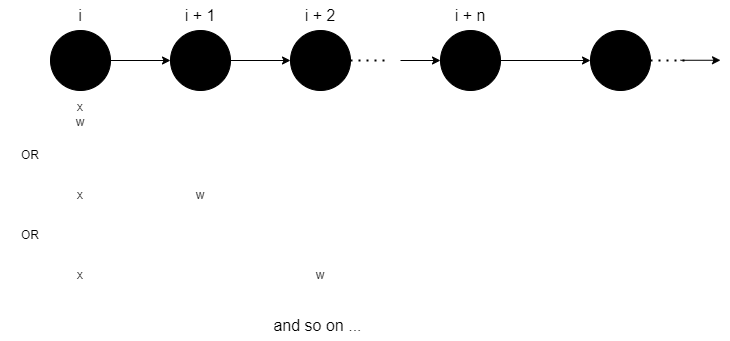
\includegraphics[scale=0.55]{p2.7.1.png}\\
		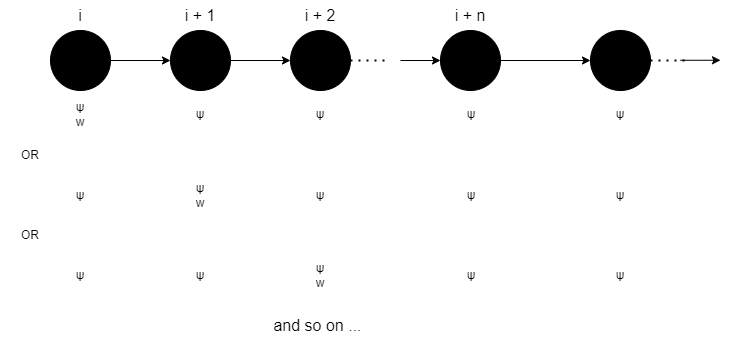
\includegraphics[scale=0.55]{p2.7.2.png}


	\item $(\Box \chi  \wedge \bigcirc	 \psi ) \rightarrow \pi \mathcal{R}  \tau $
	
	\noindent If $\chi$ is an invariant and $\psi$ is true at time $i+1$, then $\tau$ is true at all time until (and including) the time $\pi$ becomes true.\\
	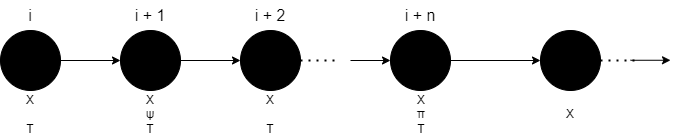
\includegraphics[scale=0.55]{p2.8.png}

	\item $\phi \rightarrow \bigcirc (\psi \wedge \chi \mathcal{U} \tau)$
	
	\noindent If $\phi$ is true at time $i$, then $\psi$ is true at time $i+1$ \
	and $\chi$ is true at at time $x+1$ up unti $\tau$ first becomes true \\
	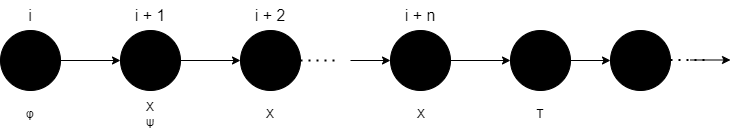
\includegraphics[scale=0.55]{p2.9.png}			

	
\end{enumerate}

\end{spacing}

\end{document}